% Preamble
\documentclass[specialist,
    substylefile = spbu_report.rtx,
    subf,href,colorlinks=true, 12pt]{disser}

% Packages
\usepackage[a4paper, includefoot,
    left=3cm, right=1.5cm,
    top=2cm, bottom=2cm,
    headsep=1cm, footskip=1cm]{geometry}
\usepackage{amsmath}
\usepackage{amssymb}
\usepackage[T2A]{fontenc}
\usepackage[utf8]{inputenc}
\usepackage[english, russian]{babel}
\usepackage{pdfpages}
\usepackage{graphicx}
\usepackage{wrapfig}
\usepackage{amsthm}
\usepackage{framed}
\usepackage{xcolor}
\usepackage{color}
\usepackage{fancyvrb}
%\usepackage{nath}
%\usepackage{cnbwp}
%\usepackage{hyperref}

\setcounter{tocdepth}{2}
\graphicspath{{./img}}

\theoremstyle{plain}
\newtheorem{statement}{Утверждение}[section]
\newtheorem{corollary}{Следствие}[statement]

\theoremstyle{definition}
\newtheorem{definition}{Определение}[section]
\newtheorem{property}{Свойство}[section]
\newtheorem{example}{Пример}[section]

\theoremstyle{remark}
\newtheorem*{remark}{Замечание}

% Document
\begin{document}

    \title{Учебная практика 3 (научно-исследовательская работа)}
    \topic{<<Tensor SSA для анализа временного ряда>>}
    \author{Хромов Никита Андреевич}
    \date{\number\year}
    \institution{
        Санкт-Петербургский государственный университет\\
        Прикладная математика и информатика
    }
    \group{20.Б04-мм}
    \sa       {Голяндина~Н.\,Э.}
    \sastatus {к.\,ф.-м.\,н., доцент}
    \city{Санкт-Петербург}
    \maketitle

    \tableofcontents


    \section{Введение}\label{sec:intro}
    Здесь должно быть введение.
    \newpage


    \section{Описание метода Tensor SSA}\label{sec:Tensor SSA-method-description}
    Дан временной ряд $F$ длины $N$
    \[F=(f_1,f_2,\ldots,f_N).\]
    На первом этапе выбираются два натуральных параметра $I, L: I+L-1\leqslant N$, по ним высчитывается третий параметр $J=N-I-L+2$.
    С учётом этих параметров строится траекторный тензор $\mathcal X$ размерности $I\times L \times J$ следующим образом
    \[\mathcal{X}_{i,l,j}=f_{i+l+j-2}\qquad i\in \overline{1:I},\, l \in\overline{1:L},\, j \in\overline{1:J}.\]
    Слои тензора будут иметь следующий вид
    \[\mathcal{X}_{,,j}=
    \begin{pmatrix}
        f_j       & f_{j+1} & \ldots & f_{j+L-1}   \\
        f_{j+1}   & \ddots  &        & \vdots      \\
        \vdots    &         & \ddots & \vdots      \\
        f_{j+I-1} & \ldots  & \ldots & f_{j+I+L-2}
    \end{pmatrix},\]
    \[\mathcal{X}_{,l,}=
    \begin{pmatrix}
        f_l       & f_{l+1} & \ldots & f_{l+J-1}   \\
        f_{l+1}   & \ddots  &        & \vdots      \\
        \vdots    &         & \ddots & \vdots      \\
        f_{l+I-1} & \ldots  & \ldots & f_{l+I+J-2}
    \end{pmatrix},\]
    \[\mathcal{X}_{i,,}=
    \begin{pmatrix}
        f_i       & f_{i+1} & \ldots & f_{i+J-1}   \\
        f_{i+1}   & \ddots  &        & \vdots      \\
        \vdots    &         & \ddots & \vdots      \\
        f_{i+L-1} & \ldots  & \ldots & f_{i+L+J-2}
    \end{pmatrix}.\]

    На втором этапе к полученному тензору применяется HOSVD~\cite{hosvd} "--- тензорное разложение,
    являющееся обобщением SVD на большие размерности.
    Результатом разложения является набор из одного тензора $\mathcal{Z}$ размерности $I\times L\times J$ и трёх
    ортогональных матриц $\mathbf{U}^{(1)},\, \mathbf{U}^{(2)},\, \mathbf{U}^{(3)}$ размерностей
    $I\times I,\, L\times L,\, J\times J$ соответственно.

    Этот набор удовлетворяет равенству
    \begin{equation}
        \mathcal{X}=\mathcal{Z}\times_1 \mathbf{U}^{(1)}\times_2 \mathbf{U}^{(2)} \times_3 \mathbf{U}^{(3)},\label{eq:trajectory-hosvd}
    \end{equation}
    где $\times_n$ "--- произведение тензора на матрицу по $n$-му измерению.
    Оно определяется следующим образом: пусть $\mathcal A$ "--- тензор размерности
    $I_1\times I_2\times\ldots\times I_K$, $\mathbf U$ "--- матрица размерности $J_n\times I_n$, тогда
    $\mathcal{A}\times_n \mathbf U$ "--- тензор размерности $I_1\times I_2\times\ldots\times I_{n-1}
    \times J_n\times I_{n+1}\times \ldots\times I_K$, который считается по формуле
    \[(\mathcal{A}\times_n \mathbf U)_{i_1 i_2\ldots i_{n-1}j_n i_{n+1}\ldots i_K} = \sum_{i_n=1}^{I_n} a_{i_1 i_2\ldots
    i_{n-1}i_n i_{n+1} \ldots i_K} u_{j_n i_n}.\]

    Обозначим за $\mathcal Z_{i_n=\alpha}$ подтензор тензора $\mathcal Z$, полученный фиксированием индекса $i_n=\alpha$.
    Тензор $\mathcal Z$ удовлетворяет следующим свойствам:
    \begin{enumerate}
        \item подтензоры $\mathcal Z_{i_n=\alpha}$ и $\mathcal Z_{i_n=\beta}$ ортогональны для всех возможных значений
        $n,\, \alpha,\, \beta: \alpha\ne\beta$:
        \[\langle\mathcal Z_{i_n=\alpha},\mathcal Z_{i_n=\beta}\rangle=0 \qquad \alpha\ne\beta,\]
        \item подтензоры расположены в порядке убывания их нормы Фробениуса:
        \[\|\mathcal Z_{i_n=1}\|\geqslant\|\mathcal Z_{i_n=2}\| \geqslant \ldots \geqslant\|\mathcal Z_{i_n=I_n}\|\]
        для всех $n\in \{1,\, 2,\, 3\}$, где $I_1=I,\, I_2=L,\, I_3=J$.
    \end{enumerate}
    \begin{definition}
        \label{def:singular-value}
        Обозначим $\sigma_i^{(n)}=\|\mathcal Z_{i_n=i}\|$ и будем называть $\sigma_i^{(n)}$ $i$-м сингулярным числом
        тензора $\mathcal X$ по измерению $n$.
    \end{definition}
    \begin{definition}
        \label{def:singular-tensor}
        Векторы $\mathbf U_i^{(n)}$ будем называть $i$-м сингулярным вектором тензора $\mathcal X$ по измерению $n$.
    \end{definition}

    Разложение~\eqref{eq:trajectory-hosvd} можно представить в виде суммы
    \[
        \mathcal{X}=\sum_{i=1}^{I} \sum_{l=1}^{L} \sum_{j=1}^{J} \mathcal{Z}_{i,l,j} \mathbf{U}^{(1)}_{i}
        \circ \mathbf{U}^{(2)}_{l} \circ \mathbf{U}^{(3)}_{j}.
    \]
    Такой вид позволяет провести третий этап "--- группировку.
    Множество индексов $\mathfrak{S}=\{1,\, 2\,\ldots,\, \min(I, L, J)\}$ разбивается по смыслу на непересекающиеся множества
    \[\mathfrak{S}=\bigcup_{k=1}^{m}\mathfrak{S}_k \qquad \mathfrak{S}_k\cap \mathfrak{S}_l =\emptyset,\, k\ne l.\]
    По каждой из групп строятся тензоры
    \begin{equation}
        \mathcal{X}^{(\mathfrak{S}_k)}=\sum_{i \in \mathfrak{S}_k} \sum_{l\in \mathfrak{S}_k} \sum_{j\in \mathfrak{S}_k}
        \mathcal{Z}_{i,l,j} \mathbf{U}^{(1)}_{i}\circ \mathbf{U}^{(2)}_{l} \circ \mathbf{U}^{(3)}_{j}.\label{eq:tens-group}
    \end{equation}

    На четвёртом этапе, по каждому тензору вида~\eqref{eq:tens-group}, полученному после этапа группировки, восстанавливается ряд.
    По соображениям построения траекторного тензора, компоненты ряда восстанавливаются усреднением вдоль плоскостей $i+l+j=\operatorname{const}$.
    Другими словами, компоненты восстановленного ряда $F^{(k)}=F^{(\mathfrak{S}_k)}$ высчитываются по формуле
    \[
        f^{(k)}_n=\frac{1}{\#\mathfrak{M}_n}\sum_{(i,l,j)\in \mathfrak{M}_n} \mathcal{X}^{(\mathfrak{S}_k)}_{i,l,j},\qquad n\in \overline{1:N},
    \]
    где $\mathfrak{M}_n=\{(i,\, l,\, j) | 1\leqslant i \leqslant I,\, 1\leqslant l \leqslant L,\, 1\leqslant j \leqslant J,\, i+l+j-2=n\}$.

    Результатом метода является набор временных рядов $F^{(1)},\ldots,\, F^{(m)}$ такой, что ${F=\sum_{k=1}^{m}F^{(k)}}$.


    \section{Свойства HOSVD}\label{sec:hosvd-properties}
    Многие свойства метода SSA являются следствиями свойств SVD\@.
    В свою очередь, многие свойства HOSVD являются аналогами свойств SVD\@.
    Таким образом, аналогичность свойств SSA и Tensor SSA может быть выведена из аналогичности некоторых свойств SVD и HOSVD\@.
    \begin{statement}
        Вычисление \emph{HOSVD} тензора $\mathcal{A}$ с $N$ размерностями сводится к вычислению \emph{SVD} на $N$ матрицах $\mathbf{A}_{(n)}$,
        которые вычисляются развёрткой тензора по $n$-му измерению.
    \end{statement}
    Другими словами, если $\mathcal{A}$ "--- тензор размерности $I_1\times I_2\times\ldots\times I_N$, то его развёртка
    по $n$-му измерению "--- это матрица $\mathbf{A}_{(n)}$ размерности $I_n\times I_{n+1}I_{n+2}\ldots I_{N}I_{1}I_{2}\ldots
    I_{n-1}$, в которой элемент $a_{i_1 i_2\ldots i_N}$ тензора содержится в строке $i_n$ и столбце с номером равным
    \[\begin{aligned}
          &(i_{n+1} - 1)I_{n+2}I_{n+3}\ldots I_{N}I_1 I_2\ldots I_{n-1} + (i_{n+2} - 1)I_{n+3}I_{n+4}\ldots I_N I_1 I_2 \ldots
          I_{n-1} + \dots \\
          &+(i_N - 1)I_1 I_2 \ldots I_{n-1} + (i_1 - 1)I_2 I_3\ldots I_{n-1} + (i_2 - 1)I_3 I_4\ldots I_{n-1} + \dots + i_{n-1}.
    \end{aligned}
    \]

    \begin{figure}[!h]
        \centering
        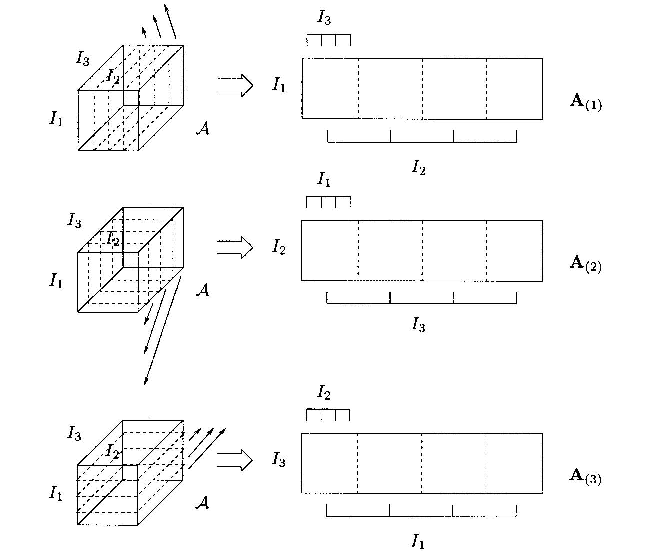
\includegraphics[width=\textwidth]{unfolding}
        \caption{Развёртка тензора $\mathcal{A}$ размерности $I_1\times I_2 \times I_3$ в матрицы $\mathbf{A}_{(1)},\,
        \mathbf{A}_{(2)},\, \mathbf{A}_{(3)}$ размерностей $I_1\times (I_2 I_3),\, I_2\times (I_3 I_1),\, I_3\times (I_1 I_2)$
            соответственно}
        \label{fig:unfolding}
    \end{figure}

    К каждой из полученных матриц применяется SVD, в результате чего получаются $N$ матриц $\mathbf{U}^{(n)}$,
    составленных из левых сингулярных векторов соответствующих развёрток.
    Затем находится тензор сингулярных чисел
    \[\mathcal{Z}=\mathcal{A}\times_1 \mathbf{U}^{(1)^\mathrm{H}}\times_2 \mathbf{U}^{(2)^\mathrm{H}}\ldots \times_N
    \mathbf{U}^{(N)^\mathrm{H}}.\]
    В результате получается искомое разложение
    \[\mathcal{A} = \mathcal{Z}\times_1 \mathbf{U}^{(1)}\times_2 \mathbf{U}^{(2)}\ldots \times_N \mathbf{U}^{(N)}.\]

    Из-за этой связи HOSVD с обычным матричным SVD для многих свойств SVD существуют аналогичные свойства HOSVD\@.
    \begin{property}[Единственность]
        \leavevmode
        \begin{enumerate}
            \item Все сингулярные числа по каждому измерению определяются однозначно.
            \item Если сингулярные числа по измерению $n$ различны, то сингулярные векторы по измерению $n$ определены
            в точности до умножения на коэффициент единичной нормы.
            Если $U_\alpha^{(n)}$ умножается на $e^{j\theta}$, то $\mathcal{Z}_{i_n=\alpha}$ должен быть умножен на обратный
            коэффициент $e^{-j\theta}$.
        \end{enumerate}
        Сингулярные векторы по измерению $n$, соответствующие одному и тому же сингулярному числу по измерению $n$,
        могут быть заменены любой унитарной линейной комбинацией.
        Соответствующие подтензоры $\{\mathcal{Z}_{i_n=\alpha}\}$ должны быть пересчитаны обратным образом.
        Формально $\mathbf{U}^{(n)}$ можно заменить на $\mathbf{U}^{(n)}\mathbf{Q}$, где $\mathbf{Q}$ "--- блочно-диагональная
        матрица, состоящая из унитарных блоков, в которой блочное разбиение соответствует разбиению $\mathbf{U}^{(n)}$
        на наборы сингулярных векторов по измерению $n$ соответствующих одинаковым сингулярным значениям по измерению $n$.
        При этом тензор $\mathcal{Z}$ должен быть заменён на $\mathcal{Z}\times_{n} \mathbf{Q}^{\mathrm{H}}$.

        В случае вещественно-значных тензоров единственность имеется в точности до знака, что соответствует
        умножению на унитарную матрицу.
    \end{property}

    \begin{property}[Обобщение]
        HOSVD тензора второго порядка сводится к его матричному SVD\@.
    \end{property}

    Перед формулировкой следующих свойств необходимо ввести определение.
    \begin{definition}[$n$-ранг]
        $n$-рангом тензора $\mathcal{A}$ называется размерность векторного пространства, порождённого векторами измерения $n$ этого тензора.
        Обозначается $R_n=\operatorname{rank}_{n}(\mathcal{A})$.
    \end{definition}

    \begin{remark}
        В отличие от матричного случая, $n$-ранги тензора порядка выше $2$ могут в общем случае отличаться.
    \end{remark}

    \begin{definition}[Тензорный ранг]
        \leavevmode
        \begin{enumerate}
            \item Говорят, что тензор $\mathcal{A}$ размерности $I_1\times I_2\times \ldots \times I_N$ имеет тензорный ранг равный $1$, если он представим в виде
            \[
                \mathcal{A}=a_1\circ a_2\circ \ldots \circ a_N,
            \]
            где $a_{k} \in \mathbb{C}^{I_k}$.
            \item Говорят, что тензор $\mathcal{A}$ имеет ранг $R$, если он представим в виде линейной комбинации $R$ тензоров
            ранга $1$, и такое $R$ минимальное.
            Обозначение: $R=\operatorname{rank}(\mathcal{A})$.
        \end{enumerate}
    \end{definition}

    \begin{remark}
        В общем случае ранг тензора $\mathcal{A}$ не равен его $n$-рангам, даже если они все равны между собой.
        Более того, всегда справедливо неравенство $\operatorname{rank}_n(\mathcal{A})\leqslant \operatorname{rank}(\mathcal{A})$.
    \end{remark}

    \begin{property}
        [Связь $n$-ранга тензора и ранга его развёртки по измерению $n$]
        Векторы размерности $n$ тензора $\mathcal{A}$ являются столбцами его развёртки по измерению $n$ и выполняется равенство
        \[\operatorname{rank}_{n}(\mathcal{A})=\operatorname{rank}(\mathbf{A}_{(n)}).\]
    \end{property}

    \begin{property}
        [Связь $n$-ранга тензора и его HOSVD]\label{property:n-rank}
        Пусть имеется HOSVD тензора $\mathcal{A}$ размерности $I_1\times I_2\times \ldots \times I_N$
        \[\mathcal{A} = \mathcal{Z}\times_1 \mathbf{U}^{(1)}\times_2\mathbf{U}^{(2)}\times_3\ldots \times_{N}\mathbf{U}^{(N)},\]
        тогда, по определению, тензор $\mathcal{Z}$ удовлетворяет свойству упорядоченности сингулярных чисел
        \[\|\mathcal{Z}_{i_n=1}\|\geqslant\|\mathcal{Z}_{i_n=2}\|\geqslant\ldots \geqslant \|\mathcal{Z}_{i_n=I_n}\|\]
        для всех $n\in \overline{1:N}$.
        Обозначим $r_n$ "--- наибольший индекс такой, что $\|\mathcal{Z}_{i_n=r_n}\|>0$.
        Тогда
        \begin{equation}
            \operatorname{rank}_n(\mathcal{A})=r_n.\label{eq:n-rank}
        \end{equation}
    \end{property}

    Все утверждения выше и их доказательства приведены в статье~\cite{hosvd}.


    \section{Свойства Tensor SSA}\label{sec:Tensor SSA-properties}
    В силу аналогичности свойств SVD и HOSVD, многие определения и свойства из теории SSA~\cite{ssa} можно перенести на тензорный случай.

    \subsection{Разделимость рядов в терминах Tensor SSA}\label{subsec:tensor-ssa-separability}
    \begin{statement}
        \label{state:separability}
        $\tilde{F}=(\tilde{f}_1,\ldots , \tilde{f}_N)$, $\hat{F}=(\hat{f}_1,\ldots , \hat{f}_N)$ "--- временные ряды длины $N$.
        Пусть ряд $F$ является суммой этих рядов.
        Траекторные тензоры рядов равны соответственно: $\tilde{\mathcal{X}},\, \hat{\mathcal{X}},\, \mathcal{X}$.
        Тогда существует сингулярное разложение тензора $\mathcal{X}$ с параметрами $I, L$, которое можно представить
        в виде суммы сингулярных разложений тензоров $\tilde{\mathcal{X}}$ и $\hat{\mathcal{X}}$ с теми же параметрами
        в том и только том случае, когда взаимно ортогональны все подряды рядов $\tilde{F}$ и $\hat{F}$
        длины $I,\, L,\, J=N-I-L+2$, то есть
        \begin{enumerate}
            \item $\tilde{f}_{k}\hat{f}_m + \ldots + \tilde{f}_{k+I-1} \hat{f}_{m+I-1}=0 \qquad \forall k,\, m\in\overline{1:N-I+1}$,
            \item $\tilde{f}_{k}\hat{f}_m + \ldots + \tilde{f}_{k+L-1} \hat{f}_{m+L-1}=0 \qquad \forall k,\, m\in\overline{1:N-L+1}$,
            \item $\tilde{f}_{k}\hat{f}_m + \ldots + \tilde{f}_{k+J-1} \hat{f}_{m+J-1}=0 \qquad \forall k,\, m\in\overline{1:N-J+1}$.
        \end{enumerate}
    \end{statement}
    \begin{proof}
        Сингулярные разложения тензоров $\mathcal{X}, \tilde{\mathcal{X}}, \hat{\mathcal{X}}$ могут быть представлены в виде
        следующих сумм:
        \[
            \begin{aligned}
                \mathcal{X}=\sum_{i=1}^{I} \sum_{l=1}^{L} \sum_{j=1}^{J} \mathcal{Z}_{i,l,j} \mathbf{U}^{(1)}_{i}
                \circ \mathbf{U}^{(2)}_{l} \circ \mathbf{U}^{(3)}_{j},\\
                \tilde{\mathcal{X}}=\sum_{i=1}^{I} \sum_{l=1}^{L} \sum_{j=1}^{J} \tilde{\mathcal{Z}}_{i,l,j}
                \tilde{\mathbf{U}}^{(1)}_{i} \circ \tilde{\mathbf{U}}^{(2)}_{l} \circ \tilde{\mathbf{U}}^{(3)}_{j},\\
                \hat{\mathcal{X}}=\sum_{i=1}^{I} \sum_{l=1}^{L} \sum_{j=1}^{J} \hat{\mathcal{Z}}_{i,l,j}
                \hat{\mathbf{U}}^{(1)}_{i} \circ \hat{\mathbf{U}}^{(2)}_{l} \circ \hat{\mathbf{U}}^{(3)}_{j}.
            \end{aligned}
        \]

        Сумма $\mathcal{X} = \sum_{i} \sum_{l} \sum_{j} \tilde{\mathcal{Z}}_{i,l,j}
        \tilde{\mathbf{U}}^{(1)}_{i} \circ \tilde{\mathbf{U}}^{(2)}_{l} \circ \tilde{\mathbf{U}}^{(3)}_{j} +
        \sum_{i} \sum_{l} \sum_{j} \hat{\mathcal{Z}}_{i,l,j} \hat{\mathbf{U}}^{(1)}_{i} \circ \hat{\mathbf{U}}^{(2)}_{l}
        \circ \hat{\mathbf{U}}^{(3)}_{j}$ является сингулярным разложением $\mathcal{X}$ в том и только том случае, когда
        пары векторов $\tilde{\mathbf{U}}^{(\sigma)}_{k},\, \hat{\mathbf{U}}^{(\sigma)}_{m}$ взаимно ортогональны
        при всех возможных значениях $\sigma, k, m$.
        Это равносильно ортогональности линейных пространств $\mathcal{L}^{(\sigma)}_{1},\, \mathcal{L}^{(\sigma)}_{2}$,
        построенных на векторах $\tilde{\mathbf{U}}^{(\sigma)}_{k}$ и $\hat{\mathbf{U}}^{(\sigma)}_{m}$ соответственно.

        Рассмотрим пространства $\mathcal{L}^{(1)}_{1},\, \mathcal{L}^{(1)}_{2}$: это пространства первых измерений
        тензоров $\tilde{\mathcal{X}}$ и $\hat{\mathcal{X}}$, то есть пространства построенные на векторах вида
        $\tilde{\mathcal{X}}_{,l,j}$ и $\hat{\mathcal{X}}_{,l,j}$ соответственно.
        Вспоминая вид тензоров $\tilde{\mathcal{X}}$ и $\hat{\mathcal{X}}$ получаем, что условие ортогональности этих
        линейных пространств равносильно первому условию из формулировки утверждения.

        Оставшиеся два условия получаются аналогично из условий ортогональности оставшихся двух пар линейных пространств.
    \end{proof}

    Из утверждения~\ref{state:separability} следует, что понятие слабой разделимости ряда из теории SSA
    применимо и к тензорному случаю.
    \begin{corollary}
        Если временные ряды $\tilde{F}$ и $\hat{F}$ длины $N$ слабо $I$- и $L$-разделимы в смысле теории \emph{SSA},
        то существует такое \emph{HOSVD} траекторного тензора $\mathcal{X}$ ряда $F=\tilde{F} + \hat{F}$, что его можно разбить
        на две части, являющиеся \emph{HOSVD} траекторных тензоров, составленных по рядам $\tilde{F}$ и $\hat{F}$.
    \end{corollary}
    \begin{remark}
        Понятие сильной разделимости можно перенести со стандартного случая на тензорный непосредственно, с поправкой на
        определение~\ref{def:singular-value} сингулярных чисел для тензора.
    \end{remark}

    \subsection{Примеры разделимости рядов в тензорном случае}\label{subsec:separation-example}
    Рассмотрим условия разделимости рядов $\tilde{F}=(\tilde{f}_{1},\, \tilde{f}_{2},\ldots,\, \tilde{f}_{N}),\, \hat{F}=
    (\hat{f}_{1},\, \hat{f}_{2},\ldots,\, \hat{f}_{N})$ в некоторых частных случаях.
    \begin{itemize}
        \item Отделимость от константного ряда

        Пусть $\tilde{f}_n=c\ne 0$ для $n\in\overline{1:N}$.
        Тогда необходимые и достаточные условия отделимости от него ряда $\hat{F}$ в смысле Tensor SSA следующие:
        \begin{enumerate}
            \item Ряд $\hat{F}$ имеет целый период $T$, и $I/T$, $L/T$, $J/T$ "--- целые;
            \item $\hat{f}_{1}+\hat{f}_2+\ldots+\hat{f}_T=0$.
        \end{enumerate}
        \begin{example}
            Ряд с элементами вида $\tilde{f}_n=\cos(2\pi n / T + \varphi)$ длины $N$ такой, что $N+2$ делится нацело на
            $T$, будет слабо отделим от константного ряда при выборе параметров $I,\, L:\: I+L< N+1$, делящихся нацело на $T$.
        \end{example}
        \item Отделимость от экспоненциального ряда

        Пусть $\tilde{f}_n=e^{\alpha n}$ для $n\in\overline{1:N}$.
        Тогда необходимые и достаточные условия отделимости от него ряда $\hat{F}$ в смысле Tensor SSA следующие:
        \begin{enumerate}
            \item Ряд $(\tilde{f}_{1}\hat{f}_{1},\, \tilde{f}_{2}\hat{f}_{2},\ldots,\, \tilde{f}_{N}\hat{f}_{N}$
            имеет целый период $T$, и $I/T$, $L/T$, $J/T$ "--- целые;
            \item $\tilde{f}_{1}\hat{f}_{1}+\tilde{f}_{2}\hat{f}_2+\ldots+\tilde{f}_{N}\hat{f}_T=0$.
        \end{enumerate}
        \begin{example}
            Ряд с элементами вида $\tilde{f}_n=e^{-\alpha n}\cos(2\pi n / T + \varphi)$ длины $N$ такой, что $N+2$ делится нацело на
            $T$, будет слабо отделим от ряда с элементами вида $\hat{f}_n=e^{\alpha n}$ при выборе параметров $I,\, L:\: I+L< N+1$, делящихся нацело на $T$.
        \end{example}
        \item Отделимость от гармонического ряда

        Пусть $\tilde{f}_n=\cos(2\pi \omega n + \varphi)$, где $0 < \omega < 1/2$, и $I, L, J > 2$.
        Положим $\hat{f}_n=\cos(2\pi \omega' n + \varphi')$,
        тогда ряд $\tilde{F}$ отделим от ряда $\hat{F}$ в смысле Tensor SSA тогда и только тогда, когда $\omega\ne\omega'$
        и $I\omega,\, I\omega',\, L\omega,\, L\omega',\, J\omega,\, J\omega'$ "--- целые числа.
    \end{itemize}

    \subsection{Ранг ряда в терминах Tensor SSA}\label{subsec:tensor-ssa-rank}
    \begin{statement}
        Пусть временной ряд $F$ имеет конечный ранг $d$ в терминах \emph{SSA}\@.
        Тогда для любых значений параметров $I$ и $L$ таких, что
        \[
            d\leqslant\min(I, L, N-I-L+2),
        \]
        количество ненулевых собственных чисел по каждому измерению в \emph{HOSVD} траекторного тензора $\mathcal{X}$,
        построенного по этому ряду с параметрами $I$ и $L$, будет равно $d$.
    \end{statement}
    Это утверждение является прямым следствием определения ранга ряда и свойства~\ref{property:n-rank} HOSVD\@.

    \begin{corollary}
        Понятие ранга ряда имеет тот же смысл в терминах Tensor SSA, что и в стандартной теории SSA, причём ряды конечного ранга
        имеют одинаковые ранги в тензорном и стандартном случаях.
    \end{corollary}


    \section{Примеры использования Tensor SSA}\label{sec:tensor-ssa-examples}
    Рассмотрим несколько примеров использования Tensor SSA для анализа временных рядов.

    \begin{example}[Разделимость синуса и константы]
        Рассмотрим ряд с элементами $f_n=3+\sin(2\pi n / 3 + \pi/3)$, где $n\in \overline{0:15}$.
        После построения траекторного тензора $\mathcal{X}$ с параметрами $I=L=6$ и его разложения получаем тензор
        сингулярных чисел $\mathcal{Z}$ и матрицы сингулярных векторов $\mathbf{U}^{(1)},\, \mathbf{U}^{(2)},\,\mathbf{U}^{(3)}$.
        Так как все размерности траекторного тензора $\mathcal{X}$ равны, его развёртки по всем
        измерениям совпадают, а значит совпадают и матрицы сингулярных векторов $\mathbf{U}^{(1)}=\mathbf{U}^{(2)}=\mathbf{U}^{(3)}=\mathbf{U}$.
        \begin{gather*}
            \mathbf{U}=
            \begin{pmatrix}
                -0.41 & 0.00  & 0.58  & 0.70  & -0.10 & 0.01  \\
                -0.41 & 0.50  & -0.29 & 0.08  & 0.62  & 0.33  \\
                -0.41 & -0.50 & -0.29 & 0.06  & 0.33  & -0.63 \\
                -0.41 & -0.00 & 0.58  & -0.70 & 0.10  & -0.01 \\
                -0.41 & 0.50  & -0.29 & -0.08 & -0.62 & -0.33 \\
                -0.41 & -0.50 & -0.29 & -0.06 & -0.33 & 0.63
            \end{pmatrix},\\
            \mathcal{Z}_{1,1,1}=-44.09,\\
            -\mathcal{Z}_{2,2,2}=\mathcal{Z}_{3,3,2}=\mathcal{Z}_{2,3,3}=\mathcal{Z}_{3,2,3}=2.60,\\
            \mathcal{Z}_{2,3,2}=\mathcal{Z}_{3,2,2}=\mathcal{Z}_{2,2,3}=-\mathcal{Z}_{3,3,3}=-4.50,\\
            \mathcal{Z}_{i,l,j}=0~\text{для всех остальных значений}~i, l, j.
        \end{gather*}

        Видно, что первый сингулярный вектор постоянен, а второй и третий "--- периодические с периодом 3.
        Кроме того, по каждому из трёх измерений количество ненулевых сингулярных чисел равно 3
        (например $\|\mathcal{Z}_{,,1}\|>\|\mathcal{Z}_{,,2}\|=\|\mathcal{Z}_{,,3}\|>0$, $\|\mathcal{Z}_{,,j}\|=0$ для всех остальных $j$).
        Исходя из этого, имеет смысл отнести индекс $\{1\}$ к константной компоненте ряда, индексы $\{2,\, 3\}$ "---
        к гармонической (синус), а остальные проигнорировать.
        После восстановления тензоров, полученных такой группировкой, получаем два ряда
        \begin{gather*}
            \hat{F}=(3,\, 3,\ldots,\, 3),\\
            \tilde{F}=(0.86,\, 0,\, -0.86,\,  0.86,\ldots,\, 0,\, -0.86,\, 0.86).
        \end{gather*}

        Таким образом, константный ряд отделился от синуса.
    \end{example}

    \begin{example}[Смешение двух косинусов]
        Рассмотрим ряд с элементами $f_n=\cos(2\pi n/3) + \cos(2\pi n/4)$, $n\in\overline{0:33}$.
        Выбрав параметры $I=L=12$, после разложения получаем тензор сингулярных значений $\mathcal{Z}$ и, в силу равенства размерностей
        траекторного тензора, равные между собой матрицы сингулярных векторов $\mathbf{U}^{(1)}=\mathbf{U}^{(2)}=\mathbf{U}^{(3)}=\mathbf{U}$.
        Тензор $\mathcal{Z}$ имеет вид тензорного блока $\mathcal{Z}'$ размерности $4\times 4\times 4$, окаймлённого нулями, в
        котором уже нельзя выделить блочно-диагональную структуру.
        Если рассмотреть матрицы сингулярных векторов, можно увидеть, что никакой сингулярный вектор не имеет периода равного $3$ или $4$:
        \[
            \mathbf{U}=
            \begin{pmatrix}
                0      & 0      & -0.58  & 0      & \ldots \\
                -0.18  & 0.36   & 0.14   & -0.39  & \ldots \\
                -0.17  & -0.16  & 0.43   & 0.30   & \ldots \\
                0.38   & -0.04  & -0.29  & 0.32   & \ldots \\
                0.14   & 0.002  & -0.14  & -0.54  & \ldots \\
                \vdots & \vdots & \vdots & \vdots & \ddots
            \end{pmatrix}.
        \]

        Таким образом, произошло смешение двух косинусов одинаковой амплитуды.
    \end{example}


    \section{Альтернативные тензорные разложения}\label{sec:other-decomp}
    Помимо HOSVD, существует ещё один тип тензорных разложений: ранговое разложение тензора.
    Идея заключается в представлении тензора $\mathcal{A}$ в виде линейной комбинации $R$ тензоров ранга $1$, где $R=\operatorname{rank}(\mathcal{A})$.
    Однако нахождение этого ранга в общем случае является NP-трудной задачей~\cite{NP-hard}.
    CANDECOMP-PARAFAC "--- итерационный метод рангового разложения тензора, который по параметру $K$ считает наилучшее приближение
    входного тензора суммой $K$ тензоров ранга $1$.
    Заметим, что из-за отсутствия каких-либо требований к ортогональности в определении рангового разложения тензора,
    многие свойства, верные в теории SSA, потеряют справедливость при использовании этого разложения.

    Рассмотрим ряды $\tilde{f}_n=3,\, \hat{f}_n=\sin(2\pi n / 3)$, $n \in \overline{0:15}$.
    Построим по этим рядам траекторные тензоры с параметрами $I=L=6$.
    Тогда ранг траекторного тензора $\tilde{\mathcal{X}}$, соответствующего константному ряду, равен $1$, так как его
    можно представить в виде
    \[
        \tilde{\mathcal{X}} = 3 X\circ X \circ X,
    \]
    где $X=(1,\, 1,\, 1,\, 1,\, 1,\, 1)$.
    Ранг траекторного тензора $\hat{\mathcal{X}}$, соответствующего синусу, равен $3$, так как его можно представить в виде
    \[
        \hat{\mathcal{X}}=\sum_{k=1}^{3}\lambda_i X_i \circ Y_i\circ Z_i,
    \]
    где
    \begin{gather*}
        \lambda_1 =160.56,\, \lambda_2 =65.69,\, \lambda_3 =123.76,\\
        \mathbf{X}=[X_1,\, X_2,\, X_3] =
        \begin{pmatrix}
            -0.16 & 0.25  & 0.06  \\
            0.25  & -0.06 & -0.25 \\
            -0.09 & -0.19 & 0.19  \\
            -0.16 & 0.25  & 0.06  \\
            0.25  & -0.06 & -0.25 \\
            -0.09 & -0.19 & 0.19
        \end{pmatrix},\\
        \mathbf{Y}=[Y_1,\, Y_2,\, Y_3] =
        \begin{pmatrix}
            -0.25 & -0.15 & 0.21  \\
            0.18  & -0.10 & -0.25 \\
            0.07  & 0.25  & 0.04  \\
            -0.25 & -0.15 & 0.21  \\
            0.18  & -0.10 & -0.25 \\
            0.07  & 0.25  & 0.04
        \end{pmatrix},\\
        \mathbf{Z}=[Z_1,\, Z_2,\, Z_3] =
        \begin{pmatrix}
            -0.10 & -0.25 & -0.01 \\
            0.25  & 0.12  & -0.24 \\
            -0.15 & 0.13  & 0.25  \\
            -0.10 & -0.25 & -0.01 \\
            0.25  & 0.12  & -0.24 \\
            -0.15 & 0.13  & 0.25
        \end{pmatrix},
    \end{gather*}
    притом точных приближений двумя тензорами ранга $1$ нет.

    Траекторный тензор ряда $f_n=\tilde{f}_n+\hat{f}_n$, построенный с параметрами $I=L=6$ представим в виде суммы
    \[
        \mathcal{X}=\sum_{k=1}^{4}\lambda_i X_i \circ Y_i\circ Z_i,
    \]
    где
    \begin{gather*}
        \lambda_1 =320.17,\, \lambda_2 =120.97,\, \lambda_3 =209.38,\, \lambda_4=648\\
        \mathbf{X}=[X_1,\, X_2,\, X_3,\, X_4] =
        \begin{pmatrix}
            -0.25 & -0.25 & 0.25 & -0.17 \\
            0.11 & 0.25 & -0.04 & -0.17 \\
            0.14 & 0.00 & -0.21 & -0.17 \\
            -0.25 & -0.25 & 0.25 & -0.17 \\
            0.11 & 0.25 & -0.04 & -0.17 \\
            0.14 & 0.00 & -0.21 & -0.17
        \end{pmatrix},\\
        \mathbf{Y}=[Y_1,\, Y_2,\, Y_3,\, Y_4] =
        \begin{pmatrix}
            0.25 & -0.25 & -0.25 & -0.17 \\
            -0.08 & 0.21 & -0.00 & -0.17 \\
            -0.17 & 0.04 & 0.25 & -0.17 \\
            0.25 & -0.25 & -0.25 & -0.17 \\
            -0.08 & 0.21 & -0.00 & -0.17 \\
            -0.17 & 0.04 & 0.25 & -0.17
        \end{pmatrix},\\
        \mathbf{Z}=[Z_1,\, Z_2,\, Z_3,\, Z_4] =
        \begin{pmatrix}
            -0.00 & -0.14 & -0.08 & 0.17 \\
            -0.25 & -0.11 & 0.25 & 0.17 \\
            0.25 & 0.25 & -0.17 & 0.17 \\
            -0.00 & -0.14 & -0.08 & 0.17 \\
            -0.25 & -0.11 & 0.25 & 0.17 \\
            0.25 & 0.25 & -0.17 & 0.17
        \end{pmatrix},
    \end{gather*}
    притом точных приближений тремя тензорами ранга $1$ нет.

    По виду векторов видно, что четвёртая компонента разложения соответствует константному ряду, а остальные три имеют период равный $3$.
    Таким образом, несмотря на отсутствие ограничений на ортогональность в определении ранговых разложений тензора, наблюдается
    отделимость константного ряда от периодического ряда при наличии условий слабой разделимости в терминах SSA\@.
    Однако понятия ранга в терминах SSA и в терминах CP различаются, так как в терминах SSA синус с периодом $3$ имеет ранг $2$, а в
    терминах рангового разложения, как показано выше, такой синус имеет ранг $3$.

    Другим недостатком CP разложения является то, что это итерационный метод, причём процесс итерации начинается
    с генерации случайной матрицы, в связи с чем на одних и тех же данных он может выдавать разные результаты, в том
    числе может как сойтись, так и нет.

    Возможно можно добиться лучших результатов, используя CP или его модификации, если строить тензор по ряду другим образом и подбирать
    другие параметры разложения.
    Этот вопрос предлагается изучить в будущих работах.
    \newpage


    \section{Заключение}\label{sec:conclusion}
    Здесь должно быть заключение.

    \bibliography{main}
    \bibliographystyle{ugost2008}

\end{document}
